\section{Approach Overview}
\label{overview:sec}

\begin{figure*}[t]
	\centering
	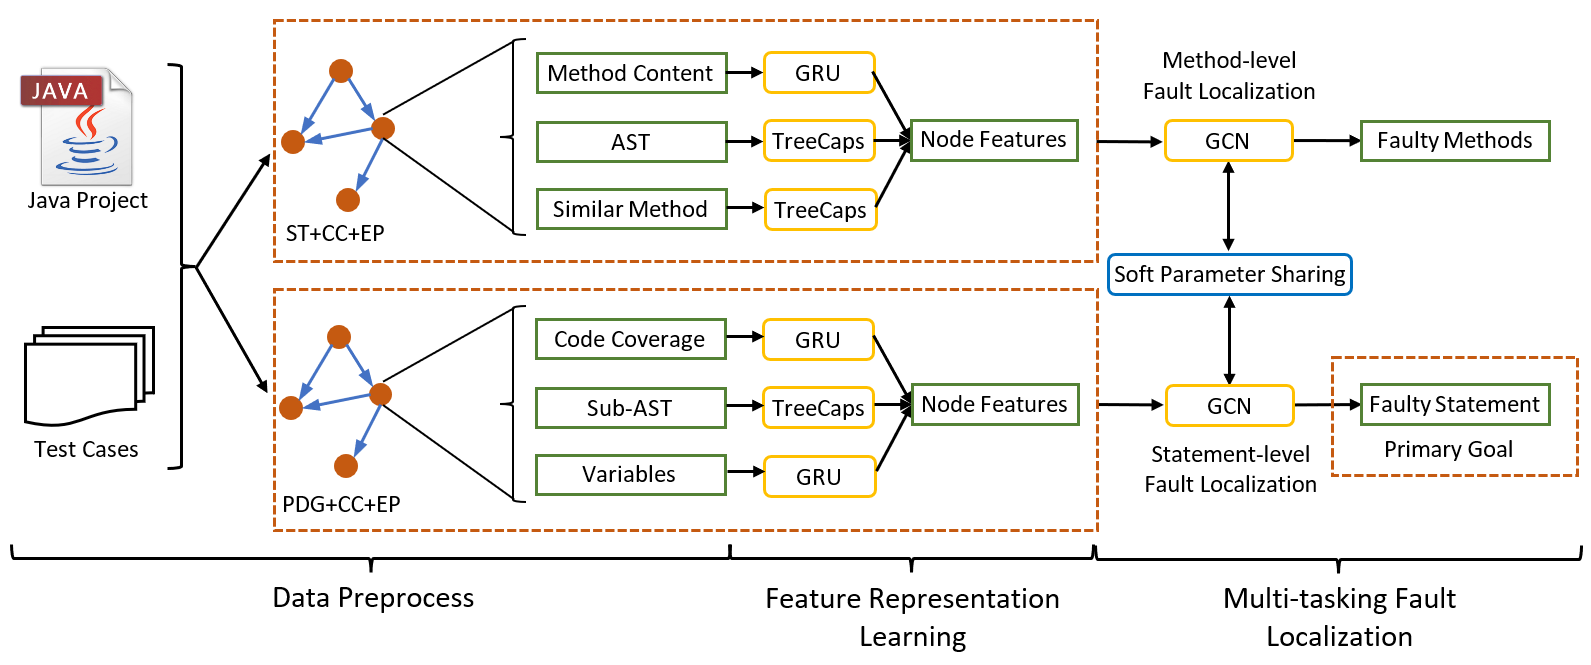
\includegraphics[width=5.6in]{graphs/overview.png}
	\caption{{\tool}: Training Process}
	\label{train-overview}
\end{figure*}

{\tool} has two main processes. Figure~\ref{train-overview} displays
the general architecture of the training process. The input of the
training process is the passing and failing test cases, as well as the
source code repository of the project under study. The output is the
parameters for the method-level pairing model (detecting co-fixed
methods) and the statement-level pairing model (detecting co-fixed
statements). The training process has three main steps:

\subsubsection*{\underline{Step 1. Feature Extraction}}
The goal of the first step is to extract the important features for FL
from the test coverage and source code (including co-changes). The
features are extracted from two levels: statements and methods. At
each level, we extract the important {\em attributes} of statements or
methods, as well as the crucial {\em relations} among them. Thus, we
use graphs to represent those attributes and relations. Let us call
them the graph-based features.

For \underline{a method $m$}, we collect as its attributes 1) method
content: the sequences of the sub-tokens of its code tokens (excluding
separators and special tokens), and 2) method structure: the Abstract
Syntax Tree (AST) of the method. For the relations among methods, we
extract the relations involving in

1) execution flow (the calling relation, i.e., $m$ calls $n$),

2) stack trace after a crash (the order relation among the methods in
the stack trace) (the dynamic information in execution paths and stack
traces has been showed to be useful in FL~\cite{icse21-fl,DeepFL}),

3) co-change relation in the project history (two methods that were
changed in the same commit are considered to have the co-change
relation),

4) similarity: we also extract the similar methods in the project that
have been buggy before in the project history. We keep only the most
similar method for each method (the similarity is measured by the one
from two sequences of sub-tokens in the two methods).

For \underline{a statement $s$}, we extract both static and dynamic
information. First, for static information, we extract the subtree in
the AST that corresponds to the statement to represent its
structure. We also extract the list of variables in the statement $s$
together with its type, forming a sequence of names and types. Second,
for the dynamic information, we encode the test coverage matrix for
$s$ as two vectors. In the first vector, the element corresponding to
the test case $i$ will be 1 if the test case covers the $s$ and 0
otherwise. In the second vector, the element for the test case $i$
will be 1 if it is passing and 0 otherwise.

At both method and statement levels, we use graphs to represent
the methods and statements, and their relations. Let us call
them method-level and statement-level feature graphs.

\subsubsection*{\underline{Step 2. Graph-based Feature Representation Learning}}

The main goal of this step is to learn the vector representations
(i.e., embeddings) for the nodes in the feature graphs built from the
step 1. The input is the method-level and statement-level feature
graphs. The output is the embeddings for the nodes in the
method-/statement-level feature graphs (the structures of the feature
graphs are un-changed).


%In this step, FixLocator aims to learn the node feature embeddings
%based on the graphs with the node features generated from step 1.
%So the input of this step is the method-level and statement-level
%graphs, and the expected output is the node embedding vectors for
%each node in each graph.
